\chapter{SM}
Følgende afsnit beskriver SM'ens hardware i de enkelte blokke, grænsefladerne derimellem samt funktionen af blokkene.

\section{Overordnet design}
Nedenfor ses det overordnede hardware blokdiagram. Herefter følger en beskrivelse af de forskellige blokke samt signaler.
\begin{figure}[H]
\centering
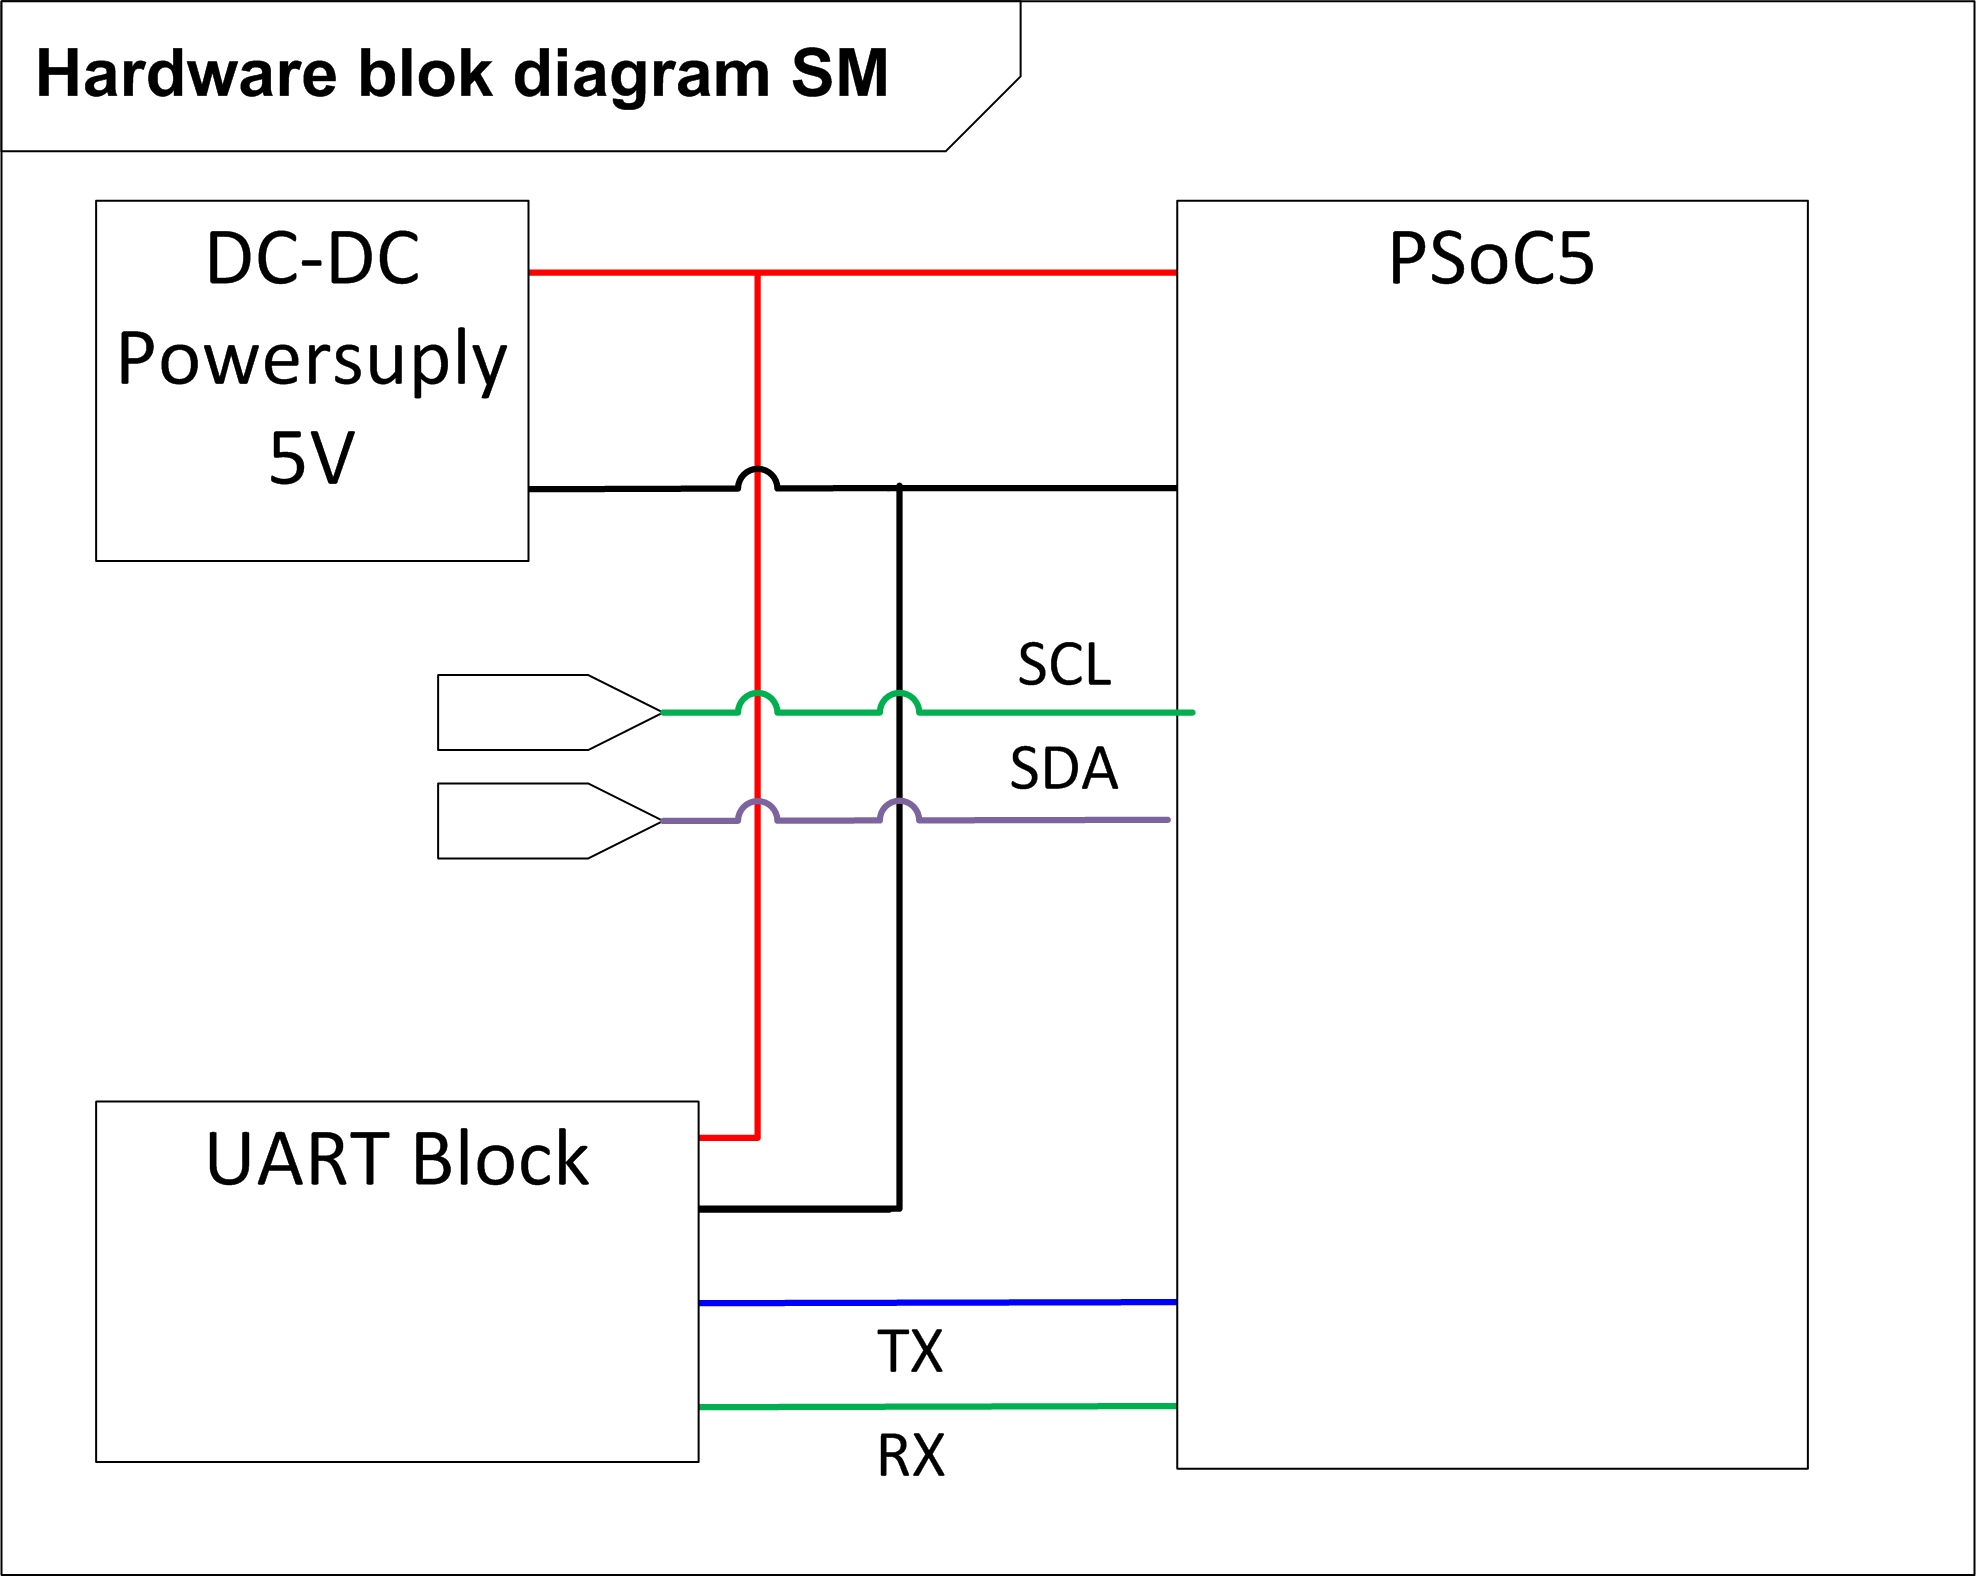
\includegraphics[width=0.5\textwidth]{billeder/SMHardware}
\caption{Overordnet blokdiagram for SM hardware}
\label{fig:HWSM}
\end{figure}
\subsection{Blokke}
Nedenfor beskrives de enkelte blokke illustreret på \textit{Figur~\ref{fig:HWSM}}
\subsubsection{PSoC5}
PSoC'en er den centrale del af VBTE'en og står for styringen af hele VBTE'en. Den består af:
\begin{itemize}
\item MicroController
\item I2C
\item Delta-Sigma ADC
\item Kontrolregister
\item UART
\end{itemize}
PSoC'en er et færdigkøbt produkt og for detaljer om de enkelte blokke heri henvises der til databladet for PSoC5.
\subsubsection{DC-DC powersuply 5V}
Se powersuply afsnittet.
\subsubsection{UART}
UART-blokken består af en levelkonverter forbundet til et DB9 stik. Levelkonverteren er af typen ST3232.
%%%%%% Nedbrydning af blokke
\section{Nedbrydning af blokke}
Nedenfor følger nedbrydningen af de enkelte blokke med henblik på at designe de enkelte dele til systemet. Nedbrydningen sker for at gøre designet nemmere og mere overskueligt.
\subsection{PSoC5}
På 